\documentclass[twoside]{book}

% Packages required by doxygen
\usepackage{fixltx2e}
\usepackage{calc}
\usepackage{doxygen}
\usepackage[export]{adjustbox} % also loads graphicx
\usepackage{graphicx}
\usepackage[utf8]{inputenc}
\usepackage{makeidx}
\usepackage{multicol}
\usepackage{multirow}
\PassOptionsToPackage{warn}{textcomp}
\usepackage{textcomp}
\usepackage[nointegrals]{wasysym}
\usepackage[table]{xcolor}

% Font selection
\usepackage[T1]{fontenc}
\usepackage[scaled=.90]{helvet}
\usepackage{courier}
\usepackage{amssymb}
\usepackage{sectsty}
\renewcommand{\familydefault}{\sfdefault}
\allsectionsfont{%
  \fontseries{bc}\selectfont%
  \color{darkgray}%
}
\renewcommand{\DoxyLabelFont}{%
  \fontseries{bc}\selectfont%
  \color{darkgray}%
}
\newcommand{\+}{\discretionary{\mbox{\scriptsize$\hookleftarrow$}}{}{}}

% Page & text layout
\usepackage{geometry}
\geometry{%
  a4paper,%
  top=2.5cm,%
  bottom=2.5cm,%
  left=2.5cm,%
  right=2.5cm%
}
\tolerance=750
\hfuzz=15pt
\hbadness=750
\setlength{\emergencystretch}{15pt}
\setlength{\parindent}{0cm}
\setlength{\parskip}{3ex plus 2ex minus 2ex}
\makeatletter
\renewcommand{\paragraph}{%
  \@startsection{paragraph}{4}{0ex}{-1.0ex}{1.0ex}{%
    \normalfont\normalsize\bfseries\SS@parafont%
  }%
}
\renewcommand{\subparagraph}{%
  \@startsection{subparagraph}{5}{0ex}{-1.0ex}{1.0ex}{%
    \normalfont\normalsize\bfseries\SS@subparafont%
  }%
}
\makeatother

% Headers & footers
\usepackage{fancyhdr}
\pagestyle{fancyplain}
\fancyhead[LE]{\fancyplain{}{\bfseries\thepage}}
\fancyhead[CE]{\fancyplain{}{}}
\fancyhead[RE]{\fancyplain{}{\bfseries\leftmark}}
\fancyhead[LO]{\fancyplain{}{\bfseries\rightmark}}
\fancyhead[CO]{\fancyplain{}{}}
\fancyhead[RO]{\fancyplain{}{\bfseries\thepage}}
\fancyfoot[LE]{\fancyplain{}{}}
\fancyfoot[CE]{\fancyplain{}{}}
\fancyfoot[RE]{\fancyplain{}{\bfseries\scriptsize Generated by Doxygen }}
\fancyfoot[LO]{\fancyplain{}{\bfseries\scriptsize Generated by Doxygen }}
\fancyfoot[CO]{\fancyplain{}{}}
\fancyfoot[RO]{\fancyplain{}{}}
\renewcommand{\footrulewidth}{0.4pt}
\renewcommand{\chaptermark}[1]{%
  \markboth{#1}{}%
}
\renewcommand{\sectionmark}[1]{%
  \markright{\thesection\ #1}%
}

% Indices & bibliography
\usepackage{natbib}
\usepackage[titles]{tocloft}
\setcounter{tocdepth}{3}
\setcounter{secnumdepth}{5}
\makeindex

% Hyperlinks (required, but should be loaded last)
\usepackage{ifpdf}
\ifpdf
  \usepackage[pdftex,pagebackref=true]{hyperref}
\else
  \usepackage[ps2pdf,pagebackref=true]{hyperref}
\fi
\hypersetup{%
  colorlinks=true,%
  linkcolor=blue,%
  citecolor=blue,%
  unicode%
}

% Custom commands
\newcommand{\clearemptydoublepage}{%
  \newpage{\pagestyle{empty}\cleardoublepage}%
}

\usepackage{caption}
\captionsetup{labelsep=space,justification=centering,font={bf},singlelinecheck=off,skip=4pt,position=top}

%===== C O N T E N T S =====

\begin{document}

% Titlepage & ToC
\hypersetup{pageanchor=false,
             bookmarksnumbered=true,
             pdfencoding=unicode
            }
\pagenumbering{roman}
\begin{titlepage}
\vspace*{7cm}
\begin{center}%
{\Large Light Controller \\[1ex]\large 1.\+0 }\\
\vspace*{1cm}
{\large Generated by Doxygen 1.8.11}\\
\end{center}
\end{titlepage}
\clearemptydoublepage
\tableofcontents
\clearemptydoublepage
\pagenumbering{arabic}
\hypersetup{pageanchor=true}

%--- Begin generated contents ---
\chapter{Class Index}
\section{Class List}
Here are the classes, structs, unions and interfaces with brief descriptions\+:\begin{DoxyCompactList}
\item\contentsline{section}{\hyperlink{structt__toggle__switch}{t\+\_\+toggle\+\_\+switch} \\*Toggle switch object has one memeber }{\pageref{structt__toggle__switch}}{}
\end{DoxyCompactList}

\chapter{File Index}
\section{File List}
Here is a list of all documented files with brief descriptions\+:\begin{DoxyCompactList}
\item\contentsline{section}{\hyperlink{toggle__switch_8h}{toggle\+\_\+switch.\+h} \\*Header file for the toggle switch module }{\pageref{toggle__switch_8h}}{}
\item\contentsline{section}{{\bfseries types.\+h} }{\pageref{types_8h}}{}
\end{DoxyCompactList}

\chapter{Class Documentation}
\hypertarget{structt__toggle__switch}{}\section{t\+\_\+toggle\+\_\+switch Struct Reference}
\label{structt__toggle__switch}\index{t\+\_\+toggle\+\_\+switch@{t\+\_\+toggle\+\_\+switch}}


Toggle switch object has one memeber.  




{\ttfamily \#include $<$toggle\+\_\+switch.\+h$>$}

\subsection*{Public Attributes}
\begin{DoxyCompactItemize}
\item 
\hyperlink{toggle__switch_8h_a808e5cd4979462d3bbe3070d7d147444}{States} {\bfseries state}\hypertarget{structt__toggle__switch_af94cce14bd44f032f240b18260f191f5}{}\label{structt__toggle__switch_af94cce14bd44f032f240b18260f191f5}

\end{DoxyCompactItemize}


\subsection{Detailed Description}
Toggle switch object has one memeber. 

defines the switch state. 

The documentation for this struct was generated from the following file\+:\begin{DoxyCompactItemize}
\item 
\hyperlink{toggle__switch_8h}{toggle\+\_\+switch.\+h}\end{DoxyCompactItemize}

\chapter{File Documentation}
\hypertarget{toggle__switch_8h}{}\section{toggle\+\_\+switch.\+h File Reference}
\label{toggle__switch_8h}\index{toggle\+\_\+switch.\+h@{toggle\+\_\+switch.\+h}}


Header file for the toggle switch module.  


{\ttfamily \#include \char`\"{}types.\+h\char`\"{}}\\*
Include dependency graph for toggle\+\_\+switch.\+h\+:\nopagebreak
\begin{figure}[H]
\begin{center}
\leavevmode
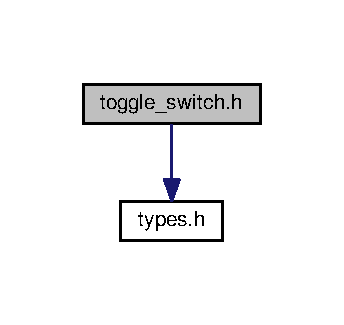
\includegraphics[width=165pt]{toggle__switch_8h__incl}
\end{center}
\end{figure}
\subsection*{Classes}
\begin{DoxyCompactItemize}
\item 
struct \hyperlink{structt__toggle__switch}{t\+\_\+toggle\+\_\+switch}
\begin{DoxyCompactList}\small\item\em Toggle switch object has one memeber. \end{DoxyCompactList}\end{DoxyCompactItemize}
\subsection*{Typedefs}
\begin{DoxyCompactItemize}
\item 
typedef struct \hyperlink{structt__toggle__switch}{t\+\_\+toggle\+\_\+switch} \hyperlink{toggle__switch_8h_aee7fad1f1831820e2cfde404e617162e}{c\+\_\+toggle\+\_\+switch}
\begin{DoxyCompactList}\small\item\em Toggle switch object has one memeber. \end{DoxyCompactList}\end{DoxyCompactItemize}
\subsection*{Enumerations}
\begin{DoxyCompactItemize}
\item 
enum \hyperlink{toggle__switch_8h_a808e5cd4979462d3bbe3070d7d147444}{States} \{ {\bfseries off}, 
{\bfseries on}
 \}\begin{DoxyCompactList}\small\item\em type definition for toggle switch states. \end{DoxyCompactList}
\end{DoxyCompactItemize}
\subsection*{Functions}
\begin{DoxyCompactItemize}
\item 
void \hyperlink{toggle__switch_8h_aba13762ac3cb6bee53cb5db6b62f1adf}{toggle\+\_\+switch\+\_\+init} (\hyperlink{toggle__switch_8h_aee7fad1f1831820e2cfde404e617162e}{c\+\_\+toggle\+\_\+switch} $\ast$p\+\_\+switch)
\begin{DoxyCompactList}\small\item\em Init function must be called right after the object has been created. \end{DoxyCompactList}\item 
void \hyperlink{toggle__switch_8h_a102b8fff165a51d25f52ee001ab67c9b}{toggle\+\_\+switch\+\_\+toggle} (\hyperlink{toggle__switch_8h_aee7fad1f1831820e2cfde404e617162e}{c\+\_\+toggle\+\_\+switch} $\ast$p\+\_\+switch)
\begin{DoxyCompactList}\small\item\em Toggle function toggles the switch state between on and off. \end{DoxyCompactList}\item 
bool \hyperlink{toggle__switch_8h_aea7c046ff1f016298e9025158d22fa5f}{toggle\+\_\+switch\+\_\+is\+\_\+on} (\hyperlink{toggle__switch_8h_aee7fad1f1831820e2cfde404e617162e}{c\+\_\+toggle\+\_\+switch} $\ast$p\+\_\+switch)
\begin{DoxyCompactList}\small\item\em is on function return the switch state. \end{DoxyCompactList}\end{DoxyCompactItemize}


\subsection{Detailed Description}
Header file for the toggle switch module. 

\begin{DoxyAuthor}{Author}
Antti Siirilä 
\end{DoxyAuthor}
\begin{DoxyDate}{Date}
15 Oct 2017 The module toggles its state between on and off whenever a toggle input is received. 
\end{DoxyDate}


\subsection{Typedef Documentation}
\index{toggle\+\_\+switch.\+h@{toggle\+\_\+switch.\+h}!c\+\_\+toggle\+\_\+switch@{c\+\_\+toggle\+\_\+switch}}
\index{c\+\_\+toggle\+\_\+switch@{c\+\_\+toggle\+\_\+switch}!toggle\+\_\+switch.\+h@{toggle\+\_\+switch.\+h}}
\subsubsection[{\texorpdfstring{c\+\_\+toggle\+\_\+switch}{c_toggle_switch}}]{\setlength{\rightskip}{0pt plus 5cm}typedef struct {\bf t\+\_\+toggle\+\_\+switch}  {\bf c\+\_\+toggle\+\_\+switch}}\hypertarget{toggle__switch_8h_aee7fad1f1831820e2cfde404e617162e}{}\label{toggle__switch_8h_aee7fad1f1831820e2cfde404e617162e}


Toggle switch object has one memeber. 

defines the switch state. 

\subsection{Enumeration Type Documentation}
\index{toggle\+\_\+switch.\+h@{toggle\+\_\+switch.\+h}!States@{States}}
\index{States@{States}!toggle\+\_\+switch.\+h@{toggle\+\_\+switch.\+h}}
\subsubsection[{\texorpdfstring{States}{States}}]{\setlength{\rightskip}{0pt plus 5cm}enum {\bf States}}\hypertarget{toggle__switch_8h_a808e5cd4979462d3bbe3070d7d147444}{}\label{toggle__switch_8h_a808e5cd4979462d3bbe3070d7d147444}


type definition for toggle switch states. 

Possible state values are off and on 

\subsection{Function Documentation}
\index{toggle\+\_\+switch.\+h@{toggle\+\_\+switch.\+h}!toggle\+\_\+switch\+\_\+init@{toggle\+\_\+switch\+\_\+init}}
\index{toggle\+\_\+switch\+\_\+init@{toggle\+\_\+switch\+\_\+init}!toggle\+\_\+switch.\+h@{toggle\+\_\+switch.\+h}}
\subsubsection[{\texorpdfstring{toggle\+\_\+switch\+\_\+init(c\+\_\+toggle\+\_\+switch $\ast$p\+\_\+switch)}{toggle_switch_init(c_toggle_switch *p_switch)}}]{\setlength{\rightskip}{0pt plus 5cm}void toggle\+\_\+switch\+\_\+init (
\begin{DoxyParamCaption}
\item[{{\bf c\+\_\+toggle\+\_\+switch} $\ast$}]{p\+\_\+switch}
\end{DoxyParamCaption}
)}\hypertarget{toggle__switch_8h_aba13762ac3cb6bee53cb5db6b62f1adf}{}\label{toggle__switch_8h_aba13762ac3cb6bee53cb5db6b62f1adf}


Init function must be called right after the object has been created. 

Once called the switch state is set to off. 
\begin{DoxyParams}{Parameters}
{\em $\ast$p\+\_\+switch} & toggle switch object \\
\hline
\end{DoxyParams}
\index{toggle\+\_\+switch.\+h@{toggle\+\_\+switch.\+h}!toggle\+\_\+switch\+\_\+is\+\_\+on@{toggle\+\_\+switch\+\_\+is\+\_\+on}}
\index{toggle\+\_\+switch\+\_\+is\+\_\+on@{toggle\+\_\+switch\+\_\+is\+\_\+on}!toggle\+\_\+switch.\+h@{toggle\+\_\+switch.\+h}}
\subsubsection[{\texorpdfstring{toggle\+\_\+switch\+\_\+is\+\_\+on(c\+\_\+toggle\+\_\+switch $\ast$p\+\_\+switch)}{toggle_switch_is_on(c_toggle_switch *p_switch)}}]{\setlength{\rightskip}{0pt plus 5cm}bool toggle\+\_\+switch\+\_\+is\+\_\+on (
\begin{DoxyParamCaption}
\item[{{\bf c\+\_\+toggle\+\_\+switch} $\ast$}]{p\+\_\+switch}
\end{DoxyParamCaption}
)}\hypertarget{toggle__switch_8h_aea7c046ff1f016298e9025158d22fa5f}{}\label{toggle__switch_8h_aea7c046ff1f016298e9025158d22fa5f}


is on function return the switch state. 


\begin{DoxyParams}{Parameters}
{\em $\ast$p\+\_\+switch} & toggle switch object \\
\hline
\end{DoxyParams}
\begin{DoxyReturn}{Returns}
true $<$-\/ switch is on, false $<$-\/ switch is off 
\end{DoxyReturn}
\index{toggle\+\_\+switch.\+h@{toggle\+\_\+switch.\+h}!toggle\+\_\+switch\+\_\+toggle@{toggle\+\_\+switch\+\_\+toggle}}
\index{toggle\+\_\+switch\+\_\+toggle@{toggle\+\_\+switch\+\_\+toggle}!toggle\+\_\+switch.\+h@{toggle\+\_\+switch.\+h}}
\subsubsection[{\texorpdfstring{toggle\+\_\+switch\+\_\+toggle(c\+\_\+toggle\+\_\+switch $\ast$p\+\_\+switch)}{toggle_switch_toggle(c_toggle_switch *p_switch)}}]{\setlength{\rightskip}{0pt plus 5cm}void toggle\+\_\+switch\+\_\+toggle (
\begin{DoxyParamCaption}
\item[{{\bf c\+\_\+toggle\+\_\+switch} $\ast$}]{p\+\_\+switch}
\end{DoxyParamCaption}
)}\hypertarget{toggle__switch_8h_a102b8fff165a51d25f52ee001ab67c9b}{}\label{toggle__switch_8h_a102b8fff165a51d25f52ee001ab67c9b}


Toggle function toggles the switch state between on and off. 


\begin{DoxyParams}{Parameters}
{\em $\ast$p\+\_\+switch} & toggle switch object \\
\hline
\end{DoxyParams}

%--- End generated contents ---

% Index
\backmatter
\newpage
\phantomsection
\clearemptydoublepage
\addcontentsline{toc}{chapter}{Index}
\printindex

\end{document}
